\section{\framework{}: An Agentic KG-RAG Framework}
\label{sec:kg_r1}

\subsection{Problem Definition}

KG-RAG spans many applications, including conversational assistants~\citep{chaudhuri2021grounding}, recommendation systems~\citep{wang2025knowledge}, and open-domain QA~\citep{zhu2025knowledgegraphguidedretrievalaugmented}. In this work, we instantiate and evaluate our approach on Knowledge Graph Question Answering (KGQA), which provides a grounded testbed for KG-RAG: ground-truth answers are tied to a fixed KG, evaluation is verifiable, and intermediate graph reasoning is interpretable. We now formalize knowledge graphs and KGQA tasks.


\noindent\textbf{Knowledge Graphs.} A knowledge graph (KG) is a graph-structured representation of real-world knowledge that encodes factual information as triples of entities and their relationships. We denote a KG as
\(
G=\{\,\langle e,r,e'\rangle \mid e,e'\!\in\!\mathcal{E},\ r\!\in\!\mathcal{R}\,\},
\)
where \(\mathcal{E}\) and \(\mathcal{R}\) denote the sets of entities and relations, respectively, and each triple \(\langle e,r,e'\rangle\) represents a directed edge from entity \(e\) to entity \(e'\) via relation \(r\). For example, there is an edge \texttt{\small{capital\_of}} from entity \texttt{\small{Springfield}} to entity \texttt{\small{Illinois}}.

\noindent\textbf{Knowledge Graph Question Answering (KGQA)} is a reasoning task based on KGs.
Consider a dataset \(D=\{(q, G, A_q)\}\), where \(q\) is a natural language question, \(G\) is a KG, and \(A_q\subseteq\mathcal{E}\) is the ground-truth answer set paired with the question. For each ground truth answer \(e^* \in A_q\), there exists one or more \emph{reasoning paths} in \(G\) that connect anchor entities mentioned in \(q\) to \(e^*\). A \emph{reasoning path} is a sequence of labeled edges \(r_1,\dots,r_\ell\in\mathcal{R}\) instantiated by entities \(e_0,\dots,e_\ell\) such that 
\(Z:\ e_0 \xrightarrow{r_1} e_1 \xrightarrow{r_2} \cdots \xrightarrow{r_\ell} e_\ell,
\)
where \(e_0\) is an anchor entity mentioned in \(q\) and \(e_\ell = e^* \in A_q\), and \(\mathcal{Z}(q, G, A_q)\) denotes the set of all valid reasoning paths for question \(q\) over \(G\) with respect to ground-truth answers \(A_q\). In solving KGQA, given \(q\) and \(G\), a model attempts to discover a subset of valid reasoning paths from \(\mathcal{Z}(q, G, A_q)\) and predicts \(\hat{A}_q\) based on the terminal entities of the discovered paths. The model's performance is evaluated by comparing \(\hat{A}_q\) with the ground truth \(A_q\). As an example, to answer the question ``What is the capital of the U.S. state whose largest city is Chicago?'', a valid reasoning path is\[\text{Chicago}\xrightarrow{\texttt{located\_in\_state}}\text{Illinois}\xrightarrow{\texttt{capital\_of}}\text{Springfield}.\]
This path belongs to \(\mathcal{Z}(q, G, A_q)\) and leads to the correct prediction \(\hat{A}_q=\{\text{Springfield}\}\).

\subsection{\framework{} Framework}

\begin{figure}[t]
    \centering
    \vspace{-2em}
    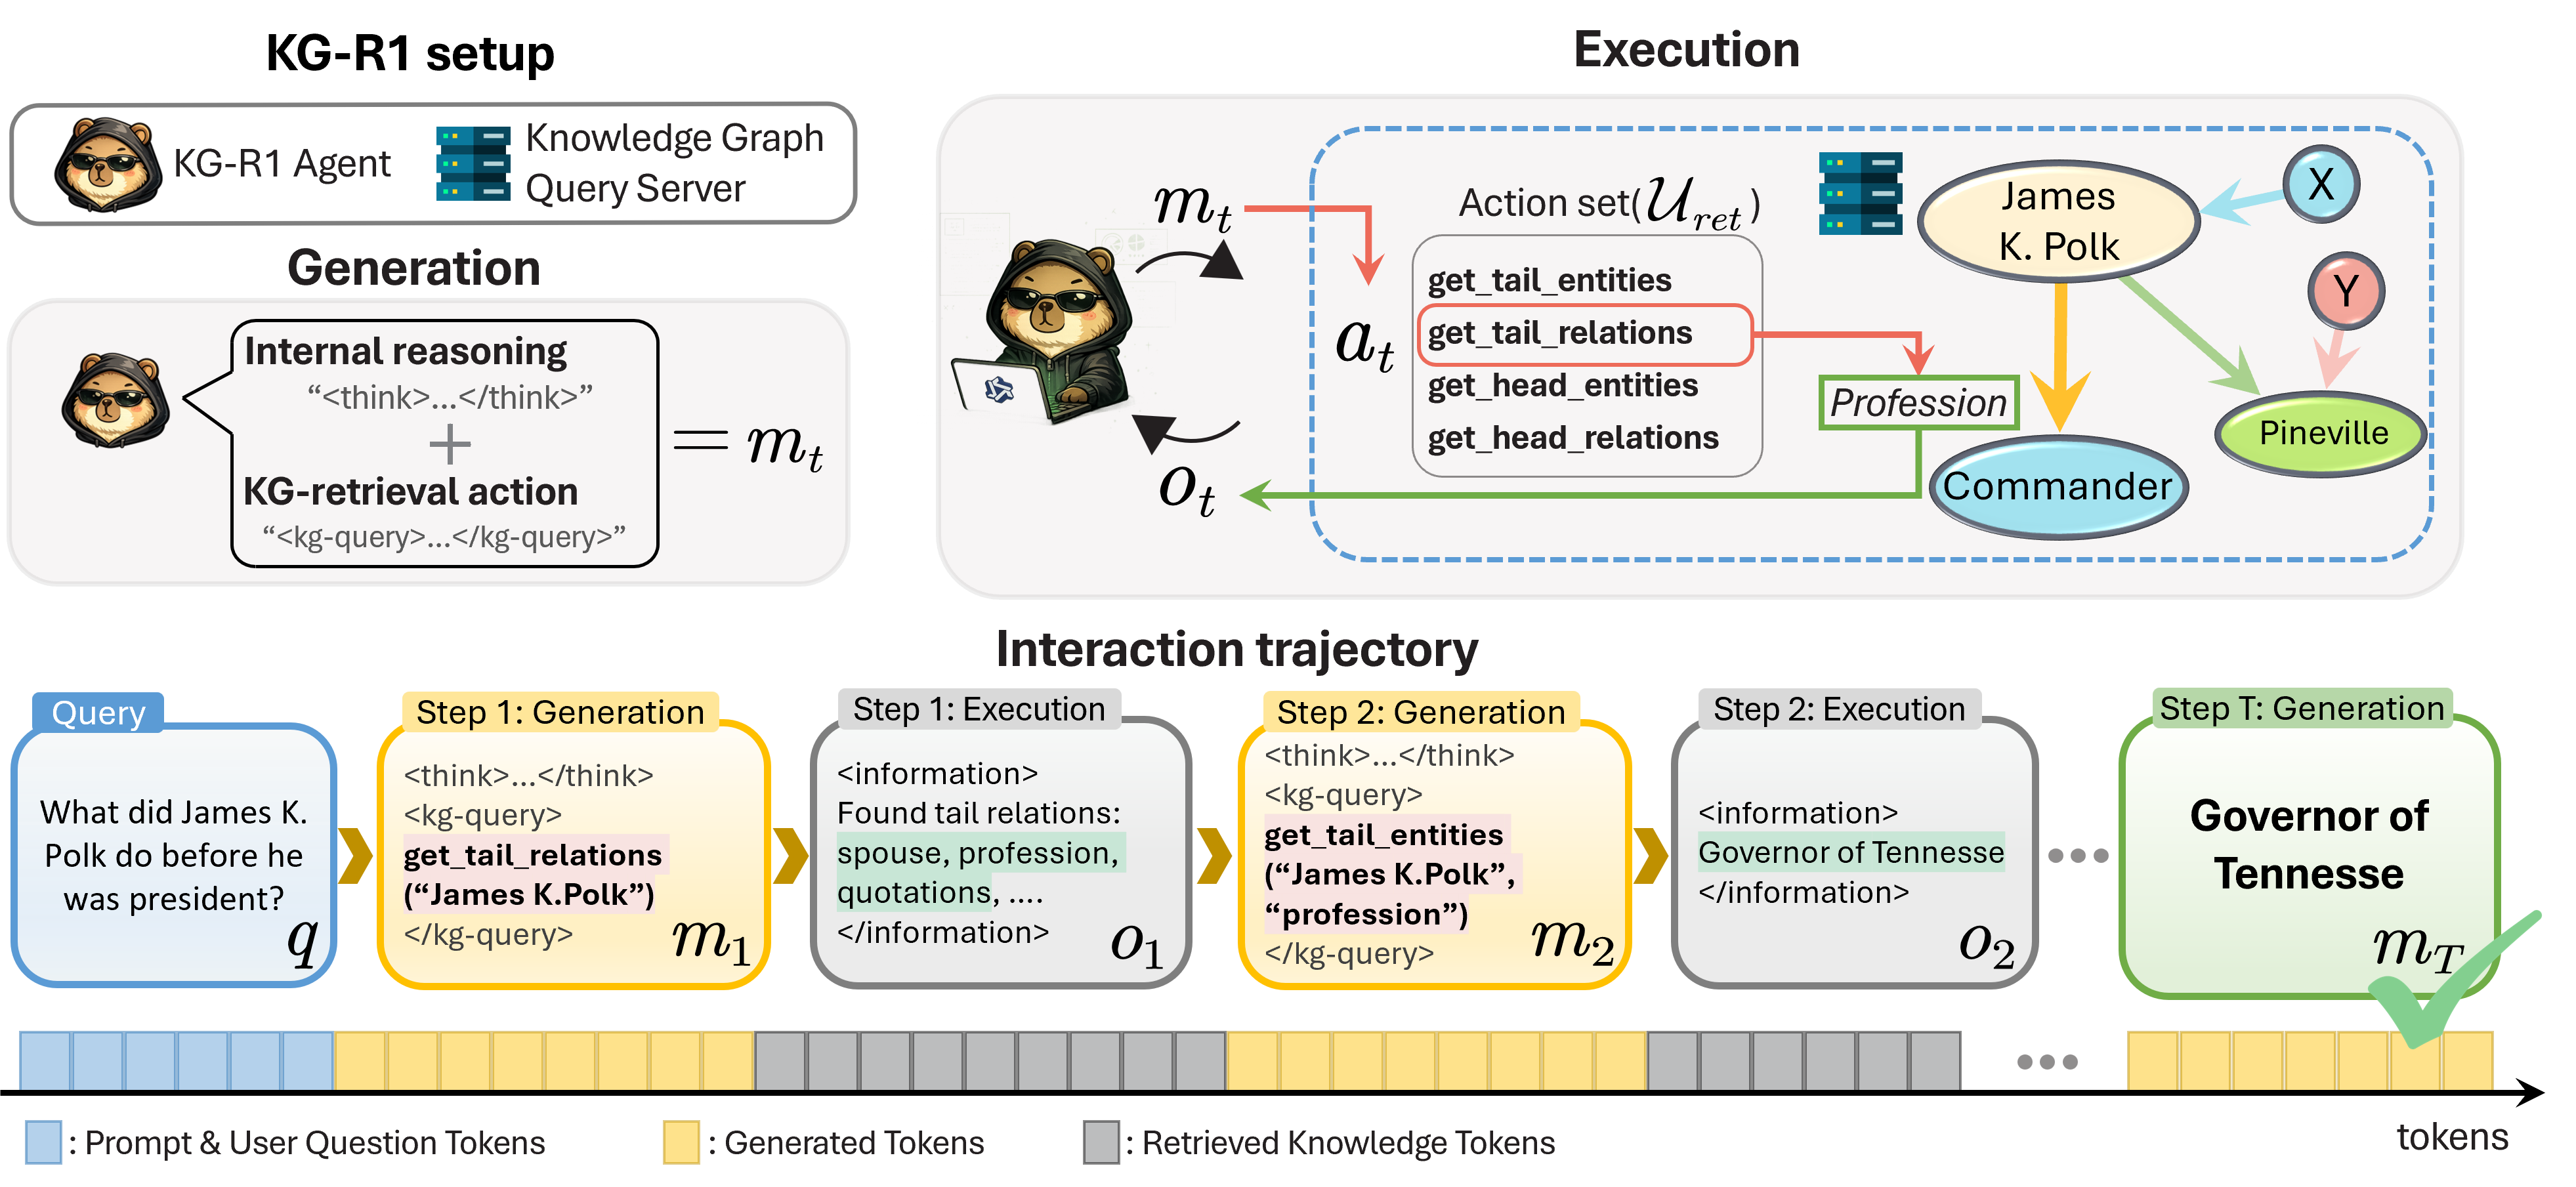
\includegraphics[width=\textwidth]{Figures/framework.png}
    \vspace{-1em}
    \caption{\framework{} framework: a single LLM agent undergoes a multi-turn generation-execution loop with a schema-agnostic KG retrieval server and responds with the final answer. }
    \label{fig3}
% \vspace{-2em}
\end{figure}

\framework{} casts KG-RAG as a multi-turn interaction with a KG interface (KG query server). We prioritize two design principles. First, we design a \emph{single-agent} architecture that simplifies deployment and enables efficient, low-cost inference. Second, we build a \emph{schema-agnostic} KG retrieval server that avoids KG-specific assumptions and remains portable across different KGs.
Given a KGQA dataset \(D=\{(q,G,A_q)\}\), we set up a KG retrieval server and a \framework{} agent. 

\noindent\textbf{KG Query Server.}
\label{subsub:kg-server}
The server hosts the knowledge graph \(G\) and provides a set of retrieval actions \(a \in \ActSet\) that enable graph traversal through 1-hop operations:
\[
\mathcal{A}_{\mathrm{ret}}
= \bigl\{ \scalebox{0.9}{$\gettailrelations,\ \getheadrelations,\ 
\gettailentities,\ \getheadentities$} \bigr\}
\]

\vspace{-2.5em}
\begin{align*}
\mathtt{get\_tail\_relations} (e)
&:= \{\, r \in \mathcal{R} \mid \exists e'\in\mathcal{E}:\ (e,r,e')\in G \,\},\\
\mathtt{get\_head\_relations} (e')
&:= \{\, r \in \mathcal{R} \mid \exists e\in\mathcal{E}:\ (e,r,e')\in G \,\},\\
\mathtt{get\_tail\_entities} (e,r)
&:= \{\, e' \in \mathcal{E} \mid (e,r,e')\in G \,\},\\
\mathtt{get\_head\_entities} (r,e')
&:= \{\, e \in \mathcal{E} \mid (e,r,e')\in G \,\}.
\end{align*}
\vspace{-1.5em}

The retrieval action set \(\ActSet\) is sufficient for \emph{realizing} any reasoning path \(Z:\ e_0 \xrightarrow{r_1} e_1 \xrightarrow{r_2} \cdots \xrightarrow{r_\ell} e_\ell\) as a finite action sequence that arrives at \(e_\ell \in A_q\) (i.e., the terminal entity is in the answer set). Forward traversal along \(Z\) is implemented by \(\mathtt{get\_tail\_entities} (e_{i-1},r_i)\) for \(i=1,\dots,\ell\) and backward traversal is implemented by \(\mathtt{get\_head\_entities} (r_i,e_i)\). 
This action design \emph{guarantees} completeness of path realization, as formalized in Remark~\ref{prop:integrity}, and provides a schema-agnostic interaction interface that enables transfer across KGs. Full formal statements and additional properties are provided in Appendix~\ref{app:kg-r1-proofs}.

\begin{restatable}[\textbf{Retrieval Action Set Completeness}]{remark}{completeness}
\label{prop:integrity}
For any reasoning path \(Z:\ e_0 \xrightarrow{r_1}\cdots\xrightarrow{r_\ell} e_\ell\) in \(G\), there exists an action sequence in \(\ActSet\) of length at most \(\ell{+}1\) whose output includes \(e_\ell\).
\end{restatable}




\noindent\textbf{\textsc{KG-R1} Agent.} 
We model a single \emph{LLM agent} that interacts with a KG query server in a multi-turn setting. The agent undergoes initialization followed by a loop of generation and execution (see Figure~\ref{fig3}). At initialization, a lightweight base LLM is configured with an instruction prompt \(p\) (see the box below for the prompt template) containing general reasoning instructions, the user question \(q\), and the KG retrieval server instructions (Table~\ref{tab:kg_server_instruction}). At each turn \(t \le H\), where $H$ is the maximum turn limit, the agent first undergoes the \textbf{generation} phase where it produces a response \(m_t\) comprising two parts: (1) an internal reasoning wrapped in \texttt{<think>...</think>}, and (2) an action, which is either a KG retrieval action wrapped in \texttt{<kg-query>...</kg-query>}, or a final answer wrapped in \texttt{<answer>...</answer>}. 

\begin{tcolorbox}[colback=white, colframe=black, title=Prompt template for \texttt{KG-R1}, boxrule=0.5pt, left=2mm, right=2mm, top=0mm, bottom=0.5mm]
\footnotesize
\label{tab:instruction_prompt}
You are a helpful assistant. Answer the given question. You can query from knowledge base provided to you to answer the question. You can query knowledge up to [H] times. You must first conduct reasoning inside \textcolor{bluetext}{$<$think$>$...$<$/think$>$}. If you need to query knowledge, you can set a query statement between \textcolor{orangetext}{$<$kg-query$>$...$<$/kg-query$>$} to query from knowledge base after \textcolor{bluetext}{$<$think$>$...$<$/think$>$}. When you have the final answer, you can output the answer inside \textcolor{redtext}{$<$answer$>$...$<$/answer$>$}. \\
KG Query Server Instruction : [{KG\_query\_server\_instruction}] \\
Question: [question]. \\
Assistant:
\end{tcolorbox}


In the following \textbf{execution} phase, we parse \(m_t\) into an \emph{action} \(a_t \in \ActSet \cup \{\answer\}\) using an exact-match parser \(\Psi\) (i.e., \(a_t=\Psi(m_t)\)). If \(a_t \in \ActSet\), executing it yields an \emph{observation} \(o_{t+1}\) (i.e., retrieved entities, relations, or an error message in case the action does not generate a valid retrieval), which is appended to the dialogue context prior to the next turn. If \(a_t=\answer\), the interaction terminates: the content inside \texttt{<answer>...</answer>} is extracted and post-processed (normalization, deduplication, and entity resolution) to produce the predicted answer set \(\hat{A}_q\). Given an interaction trajectory $\tau = (p,\,(m_1,o_1),\ldots,(m_t,o_{t}))$ with $t \leq H$, the \framework{} agent’s \emph{policy} \(\pi_\theta(m_t \mid \text{context}_t)\) is defined over token sequences \(m_t\) and governs how textual responses are generated. 

\subsection{\framework{} Training with RL}
\label{sub:kg_r1_rl}

Our goal is to learn a policy \(\pi_\theta(m_t \mid \text{context}_t)\) for the \framework{} agent that interacts with the knowledge graph $G$ over multiple turns to incrementally retrieve informative reasoning paths and ultimately produce the correct answer \(\hat{A}_q =  A_q\). We optimize this policy using reinforcement learning with a GRPO-style objective \citep{DeepSeek2025R1}, following recent advances in multi-turn agent optimization~\citep{qian2025toolrl, jin2025searchr1, zeng2025reinforcing}. An overview of the training procedure is provided in Algorithm~\ref{alg:kg_r1_training} in the \Cref{sec:kgr1_details}. %

\noindent\textbf{Reward Objective.} 
\label{subsub:Reward_Function} To effectively train the \framework{} agent, we combine verifiable \emph{turn} rewards with outcome-level \emph{global} rewards. \textbf{Turn rewards} (\(r^{\text{turn}}_{t}\)) provide local signals at each turn as the sum of three components: (i) \emph{format validity} \(v_{\mathrm{fmt}}(m_t)\) checks that \(m_t\) contains both reasoning and a well-formed action \(a_t\in\mathcal{A}\);
(ii) \emph{KG query} \(v_{\mathrm{kg}}(a_t,o_{t+1})\) checks that executing \(a_t\) yields meaningful, schema-valid retrieval in \(o_{t+1}\); and
(iii) \emph{answer consistency} \(v_{\mathrm{ans}}(m_T)\) checks the final answer’s format/consistency on the final turn. The turn rewards are computed as follows with weights $w_{fmt}$, $w_{kg}$, and $w_{ans}$: 
\begin{equation}
r^{\mathrm{turn}}_{t}
= w_{\mathrm{fmt}}\,v_{\mathrm{fmt}}(m_t)
+ w_{\mathrm{kg}}\,v_{\mathrm{kg}}(a_t,o_{t+1})
+ w_{\mathrm{ans}}\,v_{\mathrm{ans}}(m_T).
\end{equation}

\textbf{Global rewards} summarize trajectory-level outcomes as the sum of the following:
(i) a binary answer correctness signal $\mathrm{H1}$ that is $1$ if the predicted answer \(\hat{A}_q\) is included in the ground-truth answer set \(A_q\), and $0$ otherwise; and
(ii) a \emph{retrieval score} $v_{ret}$ that is \(1\) if any ground-truth entity appears anywhere in the retrieved information along the executed reasoning path, and \(0\) otherwise. 
\begin{equation}
R^{\mathrm{global}}
= w_{\mathrm{H1}}\cdot \mathrm{H1}\!\bigl(\hat{A}_q, A_q\bigr)
\;+\;
w_{\mathrm{ret}}\cdot v_{ret}
\end{equation}
\noindent\textbf{Group-relative Turn-level Credit Assignment and Optimization.} \label{subsub:rl_algo}
To assign credit across multi-turn trajectories, we adopt a group-relative, turn-level credit assignment strategy \cite{zeng2025reinforcing}. 
We collect $N$ rollouts per query $q$. For each trajectory $\tau^{(n)}$, we compute turn rewards $r^{\mathrm{turn},(n)}_t$ and a global reward $R^{\mathrm{global},(n)}$, and combine them into a per-turn return with $\lambda$ as the normalization factor:
\begin{equation}
G_t^{(n)} \;=\; r^{\mathrm{turn},(n)}_t \;+\; \lambda\,R^{\mathrm{global},(n)}.
\end{equation}
Let $\mathcal{S} \!=\! \{(n,t)\!:\! t \le T^{(n)}\}$ be the set of all turns across the $N$ rollouts. The turn-level advantage $A_t^{n}$ is calculated using a \emph{single} group baseline $\bar{G}$ that averages over $\mathcal{S}$:
\[
A_t^{(n)}=\frac{G_t^{(n)}-\bar G}{\sigma_G+\varepsilon}
\quad\text{where}\quad
\bar G=\tfrac{1}{|\mathcal S|}\!\sum_{(n,t)\in\mathcal S} G_t^{(n)},\ 
\sigma_G=\sqrt{\tfrac{1}{|\mathcal S|}\!\sum_{(n,t)\in\mathcal S}\!\big(G_t^{(n)}-\bar G\big)^2},
\]
where $\varepsilon$ is a constant for numerical stability. Intuitively, this measures each turn's contribution relative to the group average, reinforcing above-average decisions and discouraging below-average ones.

\noindent \textbf{RL update.} Using the turn-level advantage $A_t^{(n)}$, we optimize the agent's policy $\pi_\theta$ with a GRPO-style clipped objective $\mathcal{J}$:
\[
\mathcal{J}(\theta)=\mathbb{E}\!\Bigg[\sum_{n,t,i}
\Big(
\min\!\Big(\rho_{t,i}^{(n)}\widetilde{A}_{t,i}^{(n)},\ \operatorname{clip}\big(\rho_{t,i}^{(n)},1-\epsilon,1+\epsilon\big)\,\widetilde{A}_{t,i}^{(n)}\Big)
-\beta\mathrm{KL}\!\big(\pi_\theta(\cdot\mid h_{t,i}^{(n)})\|\pi_{0}(\cdot\mid h_{t,i}^{(n)})\big)
\Big)
\Bigg],
\]
where $\widetilde{A}_{t,i}^{(n)}=m_{t,i}^{(n)}A_t^{(n)}$ applies the same turn-level advantage to all tokens within a turn via a mask $m_{t,i}^{(n)}$, $\operatorname{clip}$ bounds updates to improve stability, $n$, $t$, and $i$ index trajectories, turns, and tokens, respectively. 
The current policy is $\pi_\theta$, the behavior policy $\pi_{\theta_{\text{old}}}$ is used for sampling, and $\pi_0$ is a fixed reference policy used only for KL regularization (weight $\beta$). The importance ratio
$\rho_{t,i}^{(n)}=\exp\!\big(\log \pi_\theta(y_{t,i}^{(n)}\!\mid h_{t,i}^{(n)})-\log \pi_{\theta_{\text{old}}}(y_{t,i}^{(n)}\!\mid h_{t,i}^{(n)})\big)$ corrects off-policy sampling at each token $i$. We maximize $\mathcal{J}(\theta)$ via gradient ascent. The proposed combination of structured rewards and group-relative credit assignment yields stable and informative learning signals for multi-turn decision-making, leading to improved reasoning quality and final answer correctness. We provide comprehensive ablation studies of each component of our reward design in Section~\ref{sec:exp3}.


\subsection{Cross-KG Transfer: Plug-and-Play}~\label{sec:plug_and_play}
\vspace{-.1in}

We propose a plug-and-play approach for \framework{} that enables KG-RAG to operate across different knowledge graphs without retraining. Let \(\pi_{\theta \mid \mathcal{D}}\) denote the policy of the \framework{} agent trained on a KGQA dataset \(\mathcal{D}=\{(q,G,A_q)\}\). For a new KGQA dataset \(\mathcal{D}^*=\{(q^*,G^*,A_{q^*})\}\), we replace the backend KG of the retrieval server with \(G^*\) (\emph{plug}) and evaluate \(\pi_{\theta \mid \mathcal{D}}\) on \(\mathcal{D}^*\) without any modification (\emph{play}). This approach requires no task-specific fine-tuning, data relabeling, or architectural changes. 

This plug-and-play capability stems from two design choices in \framework{}. First, the KG server exposes a schema-agnostic action set consisting solely of 1-hop retrieval operations, which are universally compatible with directed KGs. This contrasts with SPARQL-generation approaches in prior work that depend on KG-specific syntax and schema knowledge. Second, the agent’s strategy for retrieving and using KG evidence is learned in a way that is independent of any particular schema, enabling immediate transfer to new domains.



